\section{Results}

Our time-calibrated mitogenome tree (Figure \ref{UL_fig1}) reveals that the haplotypes representing our sympatric species pairs are reciprocally monophyletic, with large differences in the age of the Victoria and Kivu species pairs relative to the Mweru species pair, with the 100 best supported trees all indicating far younger divergence in Lake Victoria and Kivu. The inferred split between the two Kivu species is older than that inferred for the two Victoria species, but the 95\% HPD estimates of node height overlap for the two lakes. This indicates that it is difficult to confidently assert an older age for Kivu divergence from mitogenome data alone, although the patterns of fixed divergence across the genome we discuss below also suggest an older age for Kivu. Divergence times in both Kivu and Victoria are <5\% of the inferred divergence time for the two Mweru species, supporting our designation of old and young radiations.

Patterns of fixed divergence in the nuclear genome show a similar pattern, with Victoria exhibiting significantly less fixed divergence ($d_f$) than Kivu ($P < 0.001$, Table S1, Supporting information). Both Victoria and Kivu show much less divergence than Mweru (Figure \ref{UL_fig2}, Table S1, Supporting information). The distributions of $d_f$ suggest that what has mainly changed from the young pairs to the old pair is a rise of the genomewide background differentiation, indicating a sustained period of complete reproductive isolation in the Mweru pair. The two young pairs have nearly twice the percentage of genome blocks above the $d_f$ threshold than the older pair (Table S1, Supporting information). The 1\% and 0.1\% $d_f$ outliers in Victoria and Kivu are lower than $d_f$ in Mweru (both comparisons $P < 0.01$), but the very small number of outliers at the 0.01\% level is not distinguishable (Table S1, Supporting information).

\begin{figure}
\centering
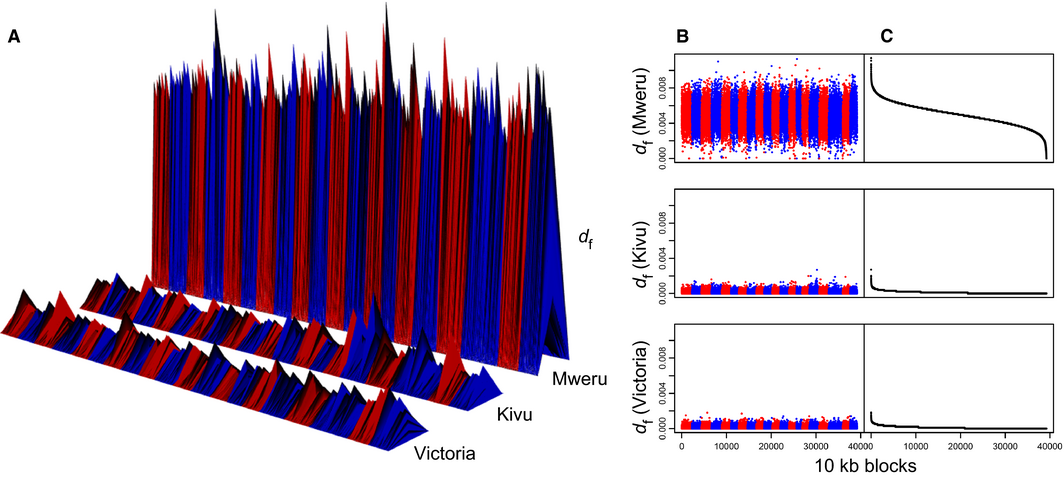
\includegraphics[width=\textwidth]{uLakes/figures/fig2}
\caption{\textbf{A, B.} Distribution of $d_f$ values in 10-kb blocks across the genome. Block heights are scaled to the maximum $d_f$ value in Lake Mweru. \textbf{C.} Genomewide $d_f$ values per 10-kb block, sorted in descending order.}
\label{UL_fig2}
\end{figure}

Comparison of outlier regions in the young Victoria and Kivu pairs revealed lower divergence than the average genomewide fixed divergence in Mweru, regardless of the outlier threshold applied (all comparisons $P < 0.01$, Table S2, Supporting information). For each species pair and for all outlier percentage levels, all $d_f$ outlier blocks also exhibited increased levels of $D_{XY}$ compared to non-$d_f$-outlier blocks (all comparisons $P < 0.0001$; Figure \ref{UL_fig3}). $d_f$ outlier blocks predicted in the Lake Victoria species pair at 1\% and 0.1\% outlier thresholds, also exhibited increased levels of $D_{XY}$ in both the Lake Kivu and the Lake Mweru pair (all comparisons $P < 0.001$), but this was not true at the 0.01\% outlier level ($P > 0.05$ for all). A similar pattern was observed for Kivu blocks in Victoria and Mweru, as well as for Mweru blocks in Kivu and Victoria (Figure \ref{UL_fig4}, Table S2).

\begin{figure}
\centering
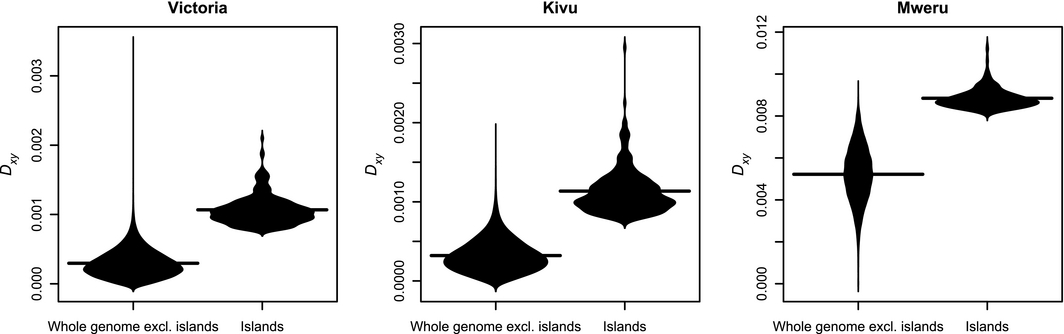
\includegraphics[width=\textwidth]{uLakes/figures/fig3}
\caption{Absolute genomic divergence patterns in three evolutionary replicates of pairs of archetypal ecomorphs of African cichlid fish (a small rock-dwelling insect picker versus a large piscivore) in the three lakes. Beanplots of $D_{XY}$ values between the whole-genome sequences excluding the top 1\% $d_f$ outlier regions and between the 1\% $d_f$ outlier regions for each species pair. Horizontal lines indicate means, and curves indicate data density. Note the different y-axis scales.}
\label{UL_fig3}
\end{figure}

\begin{figure}
\centering
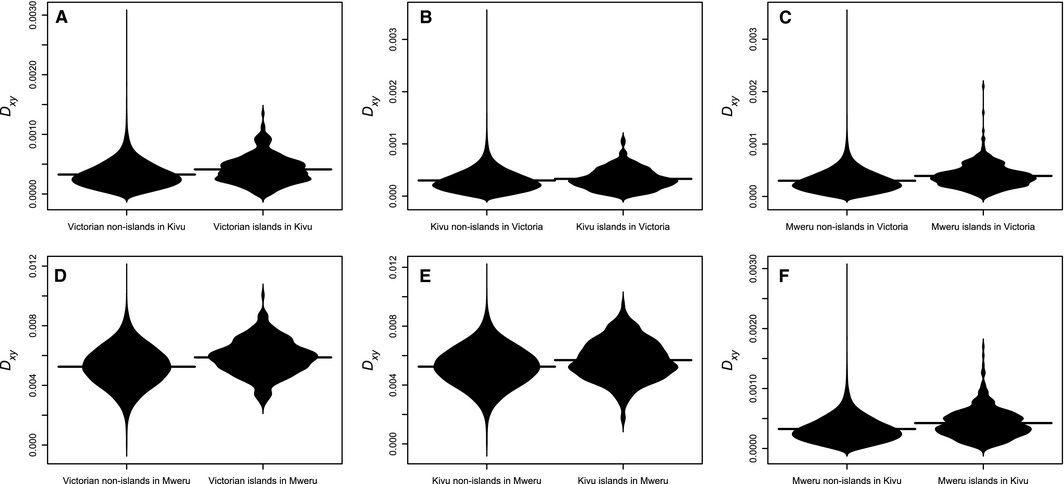
\includegraphics[width=\textwidth]{uLakes/figures/fig4}
\caption{Modest but significant extent of genomic parallelism in divergence between three evolutionary replicates of pairs of archetypal ecomorphs of African cichlid fish (a small rock-dwelling insect picker versus a large piscivore.) Beanplots of $D_{XY}$ in Kivu (\textbf{A}, \textbf{F}), Victoria (\textbf{B}, \textbf{C}) and Mweru (\textbf{D}, \textbf{E}) in regions predicted as top 1\% $d_f$ outlier regions in both other lakes, and regions not predicted as outliers in the other lakes. Horizontal lines indicate means, and curves indicate data density.}
\label{UL_fig4}
\end{figure}